%!TEX root = ../thesis.tex
%*******************************************************************************
%****************************** Second Chapter *********************************
%*******************************************************************************

\chapter{Parameter Estimation for Hidden Markov Models}

\ifpdf
    \graphicspath{{Chapter2/Figs/Raster/}{Chapter2/Figs/PDF/}{Chapter2/Figs/}}
\else
    \graphicspath{{Chapter2/Figs/Vector/}{Chapter2/Figs/}}
\fi

\section{ Expectation–Maximization algorithm}

Also abbreviated as EM algorithm is an iterative approach for computing the maximum likelihood estimates. It is used in situations where incomplete data are present therefore a part of a complete data set is hidden and we may not be able to apply straightforward analytical procedures for computing maximum likelihood estimates as in a case of complete data. 

In other words we want to find the best estimate of the parameters for which the observed sequence is the most likely. This is of great importance and efficiency for Hidden Markov models where we have a sample space of observed variables, let us denote it as $X$ and a hidden discrete sample space $Z$. We assume that there is a mapping from $X$ into $Z$, where $\forall x \in X$ is a realisation from sample space $X$ and the mapping from $X$ into $Z$ in many-one, as seen in Figure 1. We also assume that given our model the realisations $z \in Z$ are not observable directly but only as a projection from $X$ into $Z$. 

Let us also denote $\theta \in \Theta$ which is a vector of parameters of the given distribution belonging to sampling distribution $\Theta$. The aim of EM algorithm is essentially to find the best estimate of $\theta$ that maximises the likelihood function $L(\theta) = p(X|\theta)$,this is known as Maximum likelihood (ML) estimate of $\theta$. 

To visualise and apply the non-iterative approach, let us consider now the daily log returns of BTC/USDT trading pair in past 5 years. If we plot the histogram we may see that the log-returns may asymptotically follow normal distribution. Since the probability density function in such a case is unimodal and has only one global maximum, the logarithmic transformation converts multiplicative structure into additive with the preservation of global maximum to be optimised by taking the partial derivative w.r.t. each parameter. First of all, we formulate the likelihood function of two-parametric normal distribution.
 
\begin{equation}
L(\mu,\sigma^2|x_1,...,x_N) = P(\mu,\sigma^2|x_1,...,x_N) = \prod_{i=1}^{N} \frac{1}{\sqrt{2\pi \sigma^2}} e^{-\frac{1}{2} \frac{(x_i-\mu)^2}{\sigma^2}}
\end{equation}

\begin{equation}
l(\mu,\sigma^2|x_1,...,x_N) = \ln L(\mu,\sigma^2|x_1,...,x_N) 
\end{equation}

where $x_1,...,x_N$ is a vector of log-returns of length N and $\mu$ and $\sigma^2$ are parameters to be estimated. 

\begin{equation}
l(\mu,\sigma^2|x_1,...,x_N) = -\frac{N}{2} \ln(2 \pi) - \frac{N}{2} \ln(\sigma^2) - \frac{1}{2 \sigma^2} \sum_{i=1}^{N} (x_i - \mu)^2
\end{equation}

If we now take the partial derivative w.r.t. the parameter $\mu$ and $\sigma^2$ and set it to zero we obtain the ML estimate of the parameter as follows:


\begin{gather} 
\frac{\partial}{\partial \mu} l(\mu,\sigma^2|x_1,...,x_N)  = \frac{1}{\sigma^2} (\sum_{i=1}^{N} x_i - N\mu) \\
0 = \frac{1}{\sigma^2} (\sum_{i=1}^{N} x_i - N\mu) \\
\mu_{MLE} = \frac{\sum_{i=1}^{N} x_i}{N}
\end{gather}

\begin{gather} 
\frac{\partial}{\partial \sigma^2} l(\mu,\sigma^2|x_1,...,x_N) = -\frac{N}{\sigma}+ \frac{1}{\sigma^3} \sum_{i=1}^{N} (x_i - \mu)^2 \\
0 = -\frac{N}{\sigma}+ \frac{1}{\sigma^3} \sum_{i=1}^{N} (x_i - \mu)^2 \\
\sigma^2 = \frac{\sum_{i=1}^{N} (x_i - \mu)^2}{N}
\end{gather}


Given the daily returns of BTC/USDT since 2017, ML estimate of the mean denoted by $\mu$ is 0.003 and $\sigma^2$ is 0.042. Moreover we may compare the ML fit with non-parametric estimate obtained by kernel density estimate that uses a sum of gaussian kernel functions for each sampled data point to estimate the smooth density given only data and prior bandwidth parameter $h$ set to 0.2. 

Kernel density estimate is calculated as follows:

\begin{gather} 
\rho_K(y) = \sum_{i=1}^{N} K(y - x_i;h)  \\
K(x;h) \propto e^{(-\frac{x^2}{2h^2})}
\end{gather}

where $K(x;h)$ denotes the Gaussian kernel function with bandwidth parameter $h$ and $\rho_K(y)$ is a kernel density estimate at point $y$.

\begin{figure}[h]

\begin{center}
	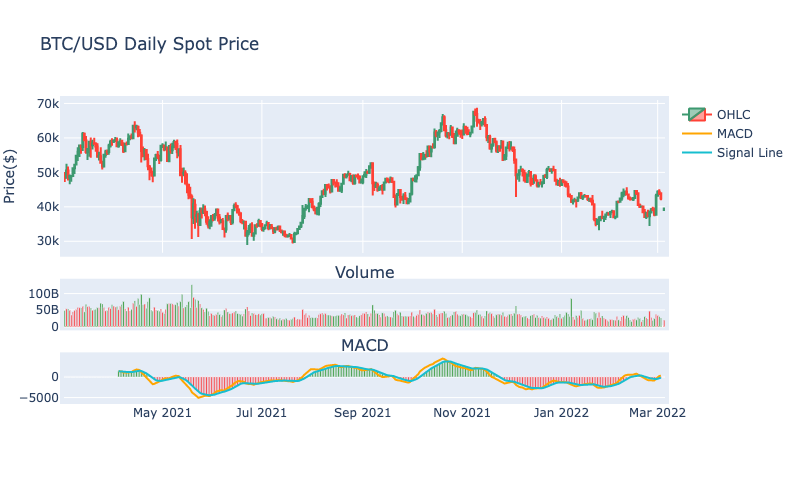
\includegraphics[width=0.9\textwidth]{MACD.png}
\end{center}

\caption{\textit{ Candlestick graph of daily spot price of BTC/USD from March 2021 to March 2022 with subplot containing two lines for MACD and Signal line and a bar chart as their difference}}

\end{figure}

Although the assumption of complete data simplifies the analytical procedure of calculating the ML estimate in closed form, it may only be used by taken in consideration observable data. The task of EM algorithm can be used to iteratively compute the most likely parameter given the data, i.e. the parameter that most likely produced such data, but since the closed form solution is available at this point, it would be redundant to use iterative procedure since both would provide the same result. Nevertheless, the iterative EM algorithm given the fully observed complete data behaves in following way:

In order to estimate the single or vector of parameters $\theta$ we use log-likelihood function:

\begin{equation}
l(\theta|X) = \ln p(X|\theta) 
\end{equation}

Since the natural logarithm is strictly monotonic increasing function the value of $\theta$ maximises the log-likelihood as well as the likelihood function. Afterwards, in a simplistic sense, the EM algorithm iterates over possible values of $\theta$ to find the best estimate, i.e. until convergence criterion is satisfied:

\begin{equation}
|l(\theta^i|X) - l(\theta^{i-1}|X)| \leq \epsilon 
\end{equation}

where the current estimate of $\theta$ in $i^{th}$ iteration is denoted by $\theta^i$ and the convergence threshold $\epsilon$. 

However, certain part of the complete data is hidden in the case of HMM, we speak about observing the incomplete part. The likelihood of the complete data is therefore a joint probability of observed and hidden part of the data. Joint probability of the complete data may also be formulated by summing over all possible values of $z$. 

\begin{equation}
l(\theta|X)  = \ln p(X|\theta) = \ln \sum_z p(X,z|,\theta)
\end{equation}

Alternatively, the goal of such an algorithm is to maximise the the loglikelihood of the complete data by estimating the optimal paramater or vector of paramaters denoted by $\theta$. Hence the marginal probability of $X$ given vector of hidden variables $Z$:

\begin{equation}
\ln p(X|\theta) = \ln \sum_{j=1}^{M} p(x, z = j|\theta)
\end{equation}

Since traditional ML procedure aims to maximise the marginal log-likelihood of complete data, part of which we do not observe, it would be unnecessarily hard to maximise. It is however possible to introduce several assumptions that will eventually suffice in providing direct solution to the maximisation problem.  Let us start by constructing the lower bound for the objective function as in Equation 2.15 that is easy to optimise with respect to parameters represented. In order to find the function $q$, we start by multiplying the marginal likelihood by $\frac{q(z)}{q(z)}$. Such expression will allow for a construction of artificial weights and with the use of Jensen's inequality:

\begin{gather}
\ln \sum_{j=1}^{M} q(z = j) \frac{p(x, z = j|\theta)}{q(z = j)}  \geq \sum_{j=1}^{M} q(z = j) \ln \frac{p(x, z = j|\theta)}{q(z = j)} = L(\theta,q) \\
\ln p(X|\theta) \geq L(\theta,q), for \forall q \in Q
\end{gather}

We have established the Jensen's inequality within the usage of concavity of logarithmic function. The constructed lower bound $l(\theta,q)$ is factorable into the expected value of the loglikelihood of complete data and entropy of probability function $q(x)$. Moreover, the maximisation of such likelihood function is completely determined by the former term since the latter is independent of $\theta$.

\begin{equation}
l(\theta,q) = \sum_{j=1}^{M} q(z = j) \ln p(x, z = j|\theta) + \sum_{j=1}^{M} q(z = j) \ln \frac{1}{q(z = j)}
\end{equation}

The optimization problem transforms into finding the function $q$ for a fixed $\theta^{k-1}$, given the k-th iteration, that maximizes $L(\theta, q)$:

\begin{equation}
q^{k} = \underset{q}{\arg\max} l(\theta, q)
\end{equation}

In other words, we want to minimise the gap between the complete data log-likelihood function $l(\theta|X)$ and incomplete data $l(\theta, q)$ with respect to function $q$. Let us now elaborate more on the gap. The final expression that we shall arrive at gives a simplifying interpretation known as Kullback-Leibler divergence (hereafter KL divergence) measures the dissimilarities between two distributions and the measure may be interpreted as a geometrical statistical distance, it also is asymmetric and non-negative. Such measure is commonly used in image or signal processing in calculation of the expected excess surprise from using $q$ as a probability distribution for our model given that the true or actual probability distribution is $p$. Substantially the measure is a difference of cross-entropy denoted by $H(p,q)$ and entropy by $H(p)$ which is always non-negative as a result of Gibb's inequality and is zero if and only if the two probability measure $p$ and $q$ are equal.

\begin{align}
D_{KL} (p || q) &= \sum_{X} p(x) \ln \frac{p(x)}{q(x)} \\
& = \sum_{x} p(x) \ln \frac{1}{q(x)} - \sum_{x} p(x) \ln \frac{1}{p(x)} \\
& = H(p,q) - H(p)
\end{align}

The lower bound introduced in Equation 2.18 and the complete data log-likelihood function $l(\theta|X)$ are obviously not the same following even intuitively from the fact that we are observing only the visible part of the data, the hidden part is still unknown. More rigorously, we have only defined the lower bound for the complete data log-likelihood function using arbitrary probability function $q(z)$, but the deeper examination of the lower bound with the use of KL divergence yields direct choice of the probability function $q(x)$. Let us decompose the lower bound in terms of the original log-likelihood function of the complete data:

\begin{align}
l(\theta,q) &= \sum_{j=1}^{M} q(z = j) \ln \frac{p(x, z = j|\theta)}{q(z = j)} \\
& = \sum_{j=1}^{M} q(z = j) \ln \frac{p(z = j|x,\theta) p(x|\theta)}{q(z = j)} \\
& = \sum_{j=1}^{M} q(z = j) \ln \frac{p(z = j|x,\theta)}{q(z = j)} + \sum_{j=1}^{M} q(z = j) \ln p(x|\theta)\\
& = -D_{KL}(q(z)||p(z|x,\theta)) + \ln p(x|\theta)
\end{align}

Now we see that the statistical distance between the two likelihood functions is determined solely by the KL divergence. In order to find the minimal distance, ideally distance of zero "length", we simply set the function $q(x)$ equal the the $p(z|X,\theta)$. This might be the posterior distribution Adame ???

\begin{equation}
\ln p(x|\theta) = l(\theta,q) + \sum_{j=1}^{M} D_{KL}(q(z=j)||p(z=j|x,\theta)) 
\end{equation}
   
The last expression is just sum of KL divergences of function $g(z_i = j)$ and the posterior distribution of the latent variable $z$ given the data and current parameter $\theta$. 

Recalling Equation 2.18, the optimisation goal lies in finding the probability distribution $q$ that maximises $L(\theta, q)$ given the current estimate of the parameter $\theta$, traditionally called as $E-step$. To extend and present a solution in finding the function $q$, following interpretation within the knowledge of Equation 2.26 is emphasised. We see that the maximum of the lower bound, i.e. of the log likelihood function, with respect to function $q(z)$ is identical to minimising the KL divergence introduced above because the first term in objective function to minimise is independent of $q(z)$: 

\begin{equation}
q^{k+1} = \underset{q}{\arg\max} L(\theta_k, q) = \underset{q}{\arg\max} (\ln p(X|\theta)  - \sum_{i=1}^{N} D_{KL} (q(z_i) || p(z_i|x_i,\theta)))
\end{equation}

To visualise E-step, let us consider arbitrary log-likelihood function of complete data $\ln p(X|\theta)$ and $l(\theta^k,q^{k+1})$ for a fixed parameter of $\theta^k$. Notice the visual representation of resulting selection of $q^{k+1}$ as a solution to E-step. Consider also the new parameter estimate of $\theta^{k+1}$ which is a part of the next step called Maximisation step, also abbreviated as M-step.

\begin{figure}[h]

\begin{center}
	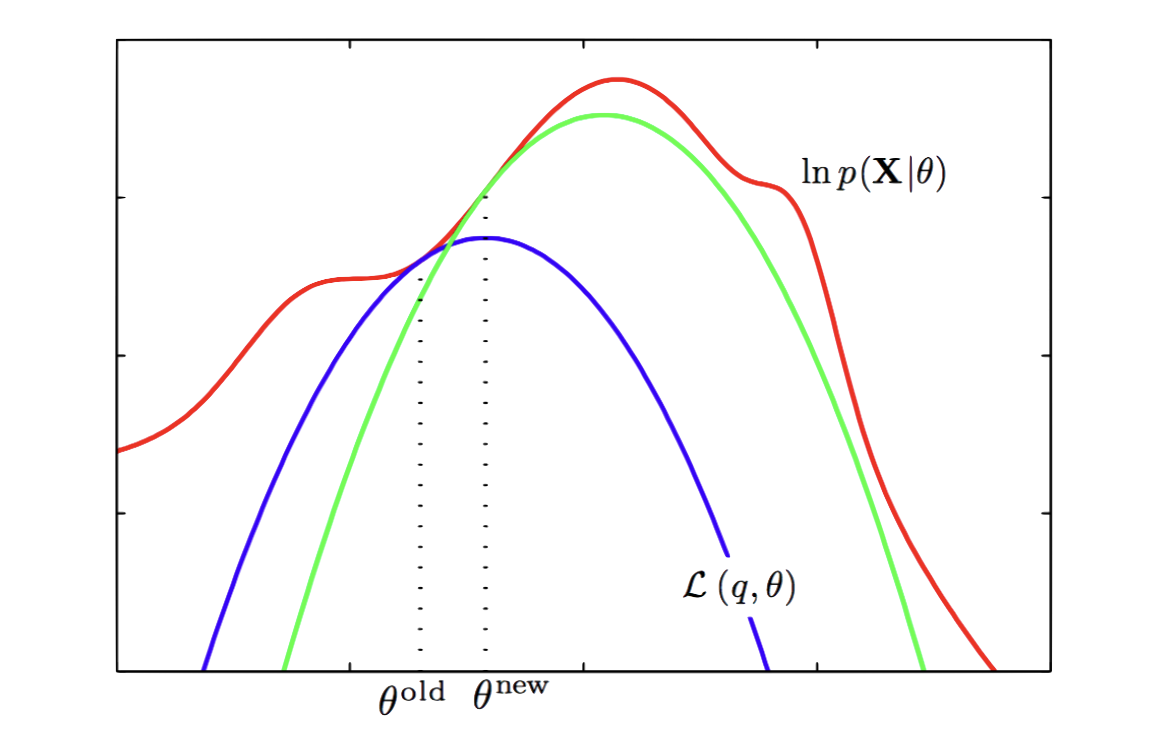
\includegraphics[width=0.9\textwidth]{Loglike.png}
\end{center}

\caption{\textit{E-step as a problem of minimisation of KL divergence represented as a gap between two likelihood functions}}

\end{figure}

Until now we have considered the optimal manner in which we compute the conditional expectation $E_{Z|X,\theta_n} [\ln P(X,z|\theta)]$ by finding the appropriate function $q$. Next step is, as is typical for coordinate descent, selection of parameter $\theta_{k+1}$ by fixing the function $q^{k+1}$ from E-step. The goal of M-step is to:

\begin{equation}
\theta^{k+1} = \underset{\theta}{\arg\max} L(\theta, q^{k+1})
\end{equation}

Thus, the EM algorithm involves two main steps:

\begin{itemize}
\item[1)] Expectation step (E-step) - choose a function q, i.e. probability distribution, that maximises $L(\theta, q)$, which may be also viewed as computing the conditional expectation $E_{Z|X,\theta_n} [\log p(X,z|\theta)]$ based on the current parameter of $\theta$.
\item[2)] Maximization step (M-step) - estimating the parameter $\theta_{k+1}$ that maximises the conditional expectation $E_{Z|X,\theta_n} [\log p(X,z|\theta)]$.
\end{itemize}

Both of these steps are repeated until convergence. 

\subsection{Baum-Welsch algorithm}

In previous section we defined Expectation-Maximization algorithm used to compute Maximum Likelihood estimates given the incomplete data, i.e. supposing that part of the data is hidden. Two main steps are called E-step and M-step which were discussed generally but we need to establish direct connection to the estimation of the Hidden Markov model parameters. We will show that former step is easily computed given variables $\alpha$, $\beta$ and $\gamma$ established in last chapter, where we defined Viterbi and Forward-Backward algorithm. These computations result in estimating the conditional probability distribution of hidden states given our observations sequence and model parameters $\mathbb{P}(z_t=i|X,\theta^k)$. The E-step in EM algorithm is just a derivation of conditional probability of particular hidden state given the data and the model parameters. In order to compute such quantity we will slightly modify the $\gamma$ definition to express it using Bayes Theorem for each observation at time t. Meaning that now we are :

\begin{equation}
\gamma_t(i) = \mathbb{P}(Z_t=i|X,\theta) = \frac{\mathbb{P}(X|Z_t=i, \theta) \mathbb{P}(Z_t = i|\theta)}{\sum_{j=1}^k \mathbb{P}(X|Z_t=j,\theta)\mathbb{P}(Z_t = j|\theta)} 
\end{equation}

where the numerator includes the conditional distribution of our data given particular hidden state $i$ and the latter term, also known as prior distribution, is our estimate of the probability distribution of hidden states. In upcoming chapter about Gaussian Mixture Models we will shown that this first term is a gaussian distribution given hidden state $i$ and the common choice for prior will be Multinomial distribution with $k$ parameters where we will stress the importance of its conjugate prior the Dirichlet distribution. Although, in case our model assumptions we use already defined variables $\alpha_t(i)$ and $\beta_t(i)$.Visually we can interpret $\gamma_t(i)$ using a similar form of a trellis as in section about Viterbi algorithm.

\begin{figure}[htbp]
\begin{center}
\begin{tikzpicture}[]
% 1st column
\node at (0,7) {$t-1$};
\node at (4,7) {$t$};
\node at (8,7) {$t+1$};

\node[state] (s1_1) at (0,6) {$z_1$};
\node[state] (s2_1) at (0,5) {$z_2$};
\node[state] (s3_1) at (0,4) {$z_3$};
\node[state] (s4_1) at (0,3) {$...$};
\node[state] (s5_1) at (0,2) {$z_N$};
% 2nd column
\node[mainstate] (s1_3) at (4,4) {$z_i$}
    edge[mainedge] (s1_1)
    edge[mainedge] (s2_1)
    edge[mainedge] (s3_1)
    edge[mainedge] (s4_1)
    edge[mainedge] (s5_1);
% 3rd column 
\node[state] (s1_5) at (8,6) {$z_1$}
    edge[mainedge]  (s1_3);
\node[state] (s2_5) at (8,5) {$z_2$}
    edge[mainedge] (s1_3);
\node[state] (s3_5) at (8,4) {$z_3$}
    edge[mainedge] (s1_3);
\node[state] (s4_5) at (8,3) {$...$}
    edge[mainedge] (s1_3);
\node[state] (s5_5) at (8,2) {$z_N$}
    edge[mainedge] (s1_3);

\end{tikzpicture}
\end{center}
\caption{Trellis interpreting the conditional probability of hidden state $i$ at time $t$ using Forward-Backward algorithm.}
\end{figure}

In Chapter 1 we denoted the transition matrix $N{\times}N$ as $A=\{a_{i,j}\}=\mathbb{P}(Z_{t}=j|Z_{t-1}=i)$, i.e. probability of transitioning to state $j$ given that we were at state $i$ at previous time ste  p. The initial distribution of hidden states $\pi_i = \mathbb{P}(Z_1=i)$, also called probability vector of length $N$, and emission matrix $N{\times}K$ defined as $B=b_i(x_t) = \mathbb{P}(X_t=x_t|Z_t=i)$, where K denotes state space, i.e. all possible outcomes, of random variables $X_t, \forall t \in T$(stochastic process???). First of all we need to specify the equation for complete data log-likelihood function for the Hidden Markov Model, which we can intuitively represent as joint probability distribution of observed and hidden data given our model parameters, i.e. $\log p(X,Z|\theta)$. Also note that here $\theta$ is considered as a vector of parameters containing initial distribution of states, transition and emission matrices, $\theta = \{\pi, A,B\}$, and is time invariant therefore:

\begin{equation}
L(\theta|x_1,...,x_T) = \pi A \prod_{t=1}^{T} b_{x_t}
\end{equation}

Time only effects the likelihood function through the emission matrix where we have to condition by the realisation of the observed process $\{X\}_{t=1}^T$, therefore $\pi A$ is a row vector and the product of column vectors. Unfortunately, the triplet of parameters does not form commuting matrices so we represent them via the sums of its elements after the logarithmic transformation below.

\begin{equation}
l(\theta|x_1,...,x_T) = \sum_{i=1}^{N}  \log \pi_i + \sum_{i,j=1}^{N} \log a_{i,j}+ \sum_{t=1}^{T} \sum_{i=1}^{N} \log b_{i,x_t}
\end{equation}

Next step according to EM algorithm is to take the expectation of the log-likelihood function above with respect to $\mathbb{P}(Z_t=i|X,\theta)$. Afterwards we may use standard tool of partially diferrentiating such function with respect to model parameters.

\begin{equation}
\mathbb{E}_{Z|X,\theta} [l(\theta|x_1,...,x_T)] = \sum_{i=1}^{N} \gamma_1(i) \log \pi_i + \sum_{t=1}^{T} \sum_{i,j=1}^{N} \gamma_t (i,j) \log a_{i,j}+ \sum_{t=1}^{T} \sum_{i=1}^{N} \gamma_t (i) \log b_{i,x_t}
\end{equation}

To summarise, the E-step of the EM algorithm in case of HMM lies in estimation of $\gamma_t(i)$ which is simply a probability of being at state $i$ given our observation sequence and model parameters. Certainly, the iterative method of EM algorithm also needs an initial guess about the model parameters, meaning the initial distribution, transition and emission matrix. Since the hidden states are assumed discrete we may express transition matrix using a stochastic (Markov) matrix introduced in Chapter 1. 

\[Include the initial paramaters\]

Note that the initial estimate of the parameters will never guarantee that we attain a global maximum of the likelihood function, therefore the optimal solution would be to initialise parameters multiple times and compare the maxima of the likelihood function. 

Once we have a formal estimate of the initial parameters, the EM algorithm performs E-step as defined above and subsequently M-step. The M-step




 





\section{Observable states}

	There is a huge number of observable variables that one could abstract from cryptocurrency market. A possibility of discrete states within the given state space is plausible and feasible, it would, given our model constraints, provide poor inference since additional information would remain hidden. Imagine a situation where our observable states are defined as a relative change in price or a sudden drop/uprise in the traded volume on the exchange. In order to discreticize our states and construct transition and emission probabilities we are forced to construct intervals that would well represent the boundaries upon which the model defines structure and predictions. 
	
Assuming that the price increase in   the idea predefined Hidden Markov Model will assume
	
	However it is much more efficient to assume continuity in our predefined observable states. It is nowadays empirically proved , as in (citace) that using technical indicators as a predictors for the future spot price yields more accurate machine learning models. As will be demonstrated each of the technical indicators can be classified into several families of indicators, such as momentum, volume, volatility and cycle indicators. For our purposes we will consider mainly momentum indicators that are calculated using Open, High, Low, Close prices (hereinafter "OHLC") and Volume indicators. There is a huge variety of technical indicators to choose from therefore the selection was made according the most used and well known indicators or their transformed versions. 

In our case we will consider following observable states that will be defined and elaborated on in the upcoming sections:

\begin{itemize}
\item[1)] Moving Average Convergence/Divergence (MACD)
\item[2)] Stochastic Oscillator
\item[3)] Chaikin Oscillator 
\item[4)] Relative Strength Index (RSI)
\item[5)] Aroon Oscillator 
\end{itemize}


\section{Moving Average Convergence Divergence}

Also knows as MACD is a trend-following momentum indicator that represents the differences between two exponential moving averages (hereinafter "EMA"). The most common and traditional moving averages are 26-period EMA and 12-period EMA. 

The indicator is often used with so called ""signal line" that is constructed as a 9-period EMA and is used as a trigger for a buy and sell signal. In practical application a trader decides to buy a stock if the signal line crosses MACD line from above and sell if it crosses from below, assuming simplistic trading strategy using only MACD. EMA also called exponentially weighted moving average is a type of moving average that differs from weighted moving average WMA by the distribution of weights to past observations. While WMA considers the linearly decreasing distribution of weights, the EMA assumes exponential decrease in weights. Furthermore it is necessary to elaborate over the values of weights because it might not always be unambiguous. WMA distributes weights chronologically and linearly, e.g. 10-period WMA gives weight 1 to the earliest observation and 10 to the most recent observation, the case within EMA is often not that simple. The weights given to each observation are computed as $(1 - \lambda)^i$ where $i \in \mathbb{N}_0$ and is bounded from above by the assumed period of interest, e.g. 3, 10, 26-period denoted as T for the sake of . As $i$ increases identically with the time lag the value of weights decreases. The important role that ought to be questioned is the parameter $\lambda$ that is defined as $\frac{k}{T+1}$ where k represents the so called "smoothing" parameter. Traders and analysts use value 2 for the smoothing parameter but the number may be defined on the interval $(0,T)$. Higher values of k mean bigger weights given to most recent observations. 

The Figure 2.1 illustrates MACD line, signal line as well as "MACD histogram" which is displayed as a bar chart indicating the difference of the former ones. Traders use such a distance to identify whether the bullish or bearish momentum is high, i.e. bigger the distances of these two lines higher the price momentum.

MACD has its unfortunate limitations that mainly arise from the non-trending moments. When the price enters sideways movement the MACD histogram signals decreases distances between MACD and signal line, the trend reversal is possible but the price moves sideways which eventually results in false positive signal. Moreover when the price moves sideways for longer periods MACD may signal too many false trend reversals. The most common practice for traders is to combine MACD signals with other indicators such as Relative Strength index (RSI) that measures overbought or oversold market. The RSI uses average price gains and losses usually over 14 periods and yields values between 0 and 100, indicating overbought market for values 70 (80) to 100 and 30 (20) to 0 for oversold market. The idea is that when the distances between MACD line and signal line increase and RSI signals overbought market the trader might consider this as a strong trend reversal signal. The idea is that signals from MACD strategy often produce false signals when price suddenly moves sideways and RSI helps to indicate the false positive signal. 

\begin{figure}[h]

\begin{center}
	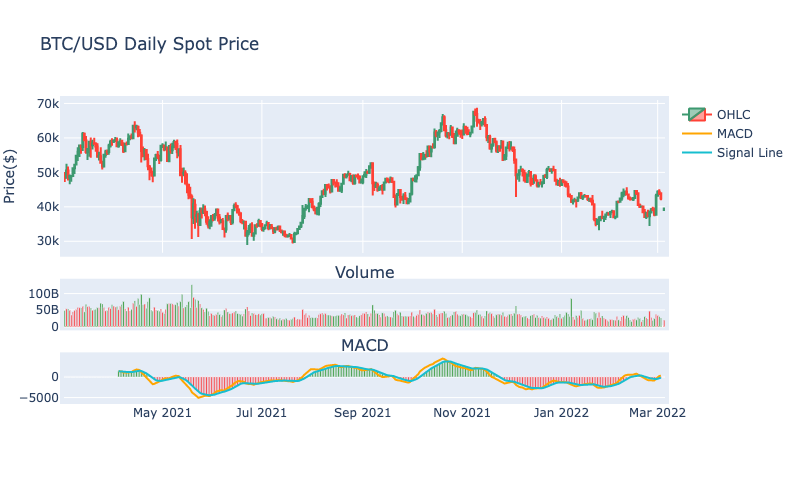
\includegraphics[width=0.9\textwidth]{MACD.png}
\end{center}

\caption{\textit{ Candlestick graph of daily spot price of BTC/USD from March 2021 to March 2022 with subplot containing two lines for MACD and Signal line and a bar chart as their difference}}

\end{figure}

\section{Stochastic Oscillator}

	A Stochastic Oscillator is a momentum indicator that compares the most recent closing price of a security with its predeceasing ones. Naturally, the range of preceding closing prices or the range of closing prices is 14 periods but it is regular that such an assumption is often edited to best fit the current needs of a trader. Also slight variation in taking the (weighted) moving average of the oscillator values is often introduced. The indicator is used to generate trading signals that refer to the current overbought state of the market, which means that the indictor values range from 0 to 100 where the values closer to the number 0 indicate oversold market and inversely values closer to 100 overbought market. 
	
Stochastic Oscillator is computed as follows:

\begin{equation}
SO_{t} = \frac{C_{t-1} - L_{14}}{H_{14} - L_{14}}
\end{equation}

where $C_{t-1}$ denotes the most recent closing price of a security, $H_{14}$ and $L_{14}$ are the highest and lowest price traded during 14-period interval respectively. $SO_{t}$ is sometimes referred to as a "fast" stochastic indicator. As said before this interval may be changed arbitrarily. Traders also developed so called "slow" Stochastic Oscillator which is defined as a 3-period moving average of $SO_{t}$. Thus when Stochastic Oscillator crosses the smooth "Slow" Stochastic Oscillator a trading signal is generated.

Considering values above 80, the indicator signals overbought market and oversold market when the value drops below 20. Although it remains to hold true that the indicator often produces false indications that may be caused by periods of time where the price remains overbought/oversold for some time and trading with respect to such oscillator may result in losses. It is rather recommended to observe the values of stochastic oscillator and use it for trend reversal indication. 

\begin{figure}[h]

\begin{center}
	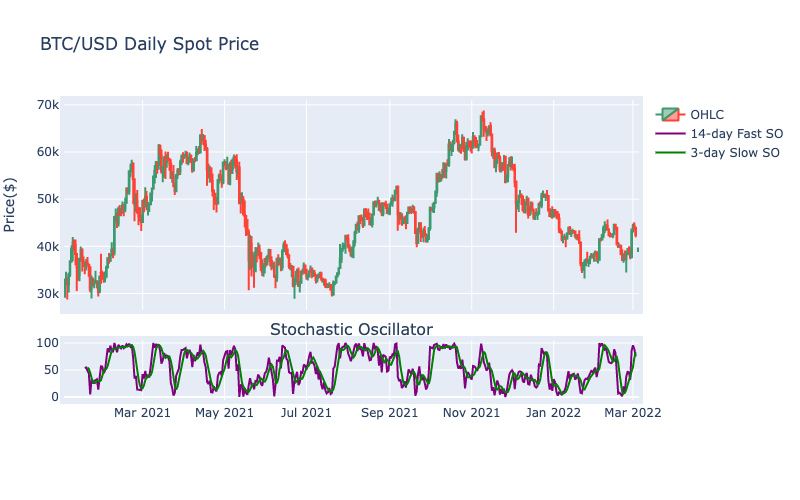
\includegraphics[width=0.9\textwidth]{Stochastic.png}
\end{center}

\caption{\textit{ Candlestick graph of daily spot price of BTC/USD from March 2021 to March 2022 with subplot with line indicating Stochastic Oscillator}}

\end{figure}

\newpage

\section{Chaikin Oscillator}

Chaikin Oscillator is a momentum based indicator of the Accumulation/Distribution Line (hereinafter "A/D line"), which is a cumulative indicator that aims to identify potential divergences between stock price and trading volume. The oscillator is calculated as a difference between 3- day and 10-day Exponential Moving Average of A/D line. 

\vspace{0.5cm}

The calculation of the Chaikin Oscillator may be broken down into several steps:
\begin{itemize}
\item[(i)] First of all we ought to calculate the Money Flow Multiplier for each time step denoted by "N".

\begin{equation}
N_{t} = \frac{(Close_{t} - Low_{t}) - (High_{t} - Close_{t})}{High_{t} - Low_{t}}
\end{equation}

\item[(ii)] Now we may multiply $N_t$ by the trading volume in given period of time to get the Money Flow Volume denoted as $M_t$. With that we recursively construct the A/D line as:

\begin{equation}
ADL_t = M_{t-1} + M_t
\end{equation}

\item[(iii)] Given the constructed A/D line, we compute the Chaikin Oscillator values as a difference of 3-day and 10-day exponential moving averages.

\begin{equation}
CO_t = \frac{\sum_{i=0}^{3} (1-\alpha)^i*Close_{t-i}}{\sum_{i=0}^{3} (1-\alpha)^i} - \frac{\sum_{i=0}^{10} (1-\beta)^i*Close_{t-i}}{\sum_{i=0}^{10} (1-\beta)^i}
\end{equation}

where we assume that the weights denoted as $\alpha$ and $\beta$ are computed as $2/(days + 1)$. Numerator as a smoothing factor is often declared as 2. However the indicator may be set to absolutely different number between 0 and 1 according to the needs and assumptions made by the trader/analyst, therefore setting the parameter close to 1 is putting more weight to the most recent price.

One way to interpret the indicator is to trade with respect to the time when the Chaikin Oscillator crosses zero from below and above which signals buy and sell signals respectively.

\end{itemize}


\begin{figure}[h]

\begin{center}
	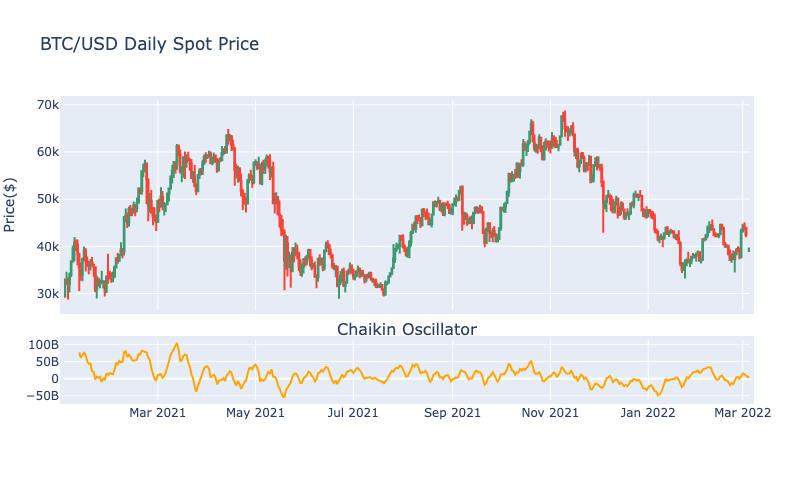
\includegraphics[width=0.9\textwidth]{Chaikin.png}
\end{center}

\caption{\textit{ Candlestick graph of daily spot price of BTC/USD from March 2021 to March 2022 with subplot indicating Chaikin Oscillator}}

\end{figure}


\section{Relative Strength Index}

Given the recent price changes Relative Strength Index measures the its magnitude in order to indicate the overbought or oversold market. In technical analysis such indicator is represented by an oscillator ranging from values 0 to 100. Empirically 
it was determined that values above 70 and below 30 signal overbought and oversold asset respectively. Therefore we may also use RSI to produce buy and sell signals from former logic, which means that when the RSI crosses 30 from below, buy signal is generated as well as sell signal in case it crosses 70 from above. We also could measure the strength and continuation of the trend for cases in which the RSI crosses value of 50. Such interpretation results from the RSI formula where the value of 50 means that the average gain equals the average loss in the last period.

The formula below explains the procedure within which the values of RSI are calculated. It is obvious that the RSI rises as the number of positive closing prices increases, i.e. the relative change in prices is positive, and falls if otherwise. The standard time interval for  the calculation is 14 preceding periods with respect to $t$, hereby denoted as $T$.

\begin{equation}
RSI_t = 100- \frac{100}{1+r_t} 
\end{equation}
 
 where r is a ratio of average gains and losses as follows:
 
\begin{equation}
 r_t = \abs{\frac{\sum_{i=1}^{T}(\frac{P_{t-i+1}}{P_{t-i}}-1)\mathbbm{1}_{[P_{t-i+1} - P_{t-i} > 0]}}{\sum_{i=1}^{T}(\frac{P_{t-i+1}}{P_{t-i}}-1) \mathbbm{1}_{[P_{t-i+1} - P_{t-i} < 0]}}}
\end{equation}

given that $P_t$ denotes the value of an asset at time $t$.

As stated before there are several drawbacks of using the RSI as a trading indicators only by itself, it happens that the price usually rises and stays overbought for a substantial period of time in times of significant and strong bullish trend. RSI as an oscillator is used as a auxiliary trading tool below the price chart:

\begin{figure}[h]

\begin{center}
	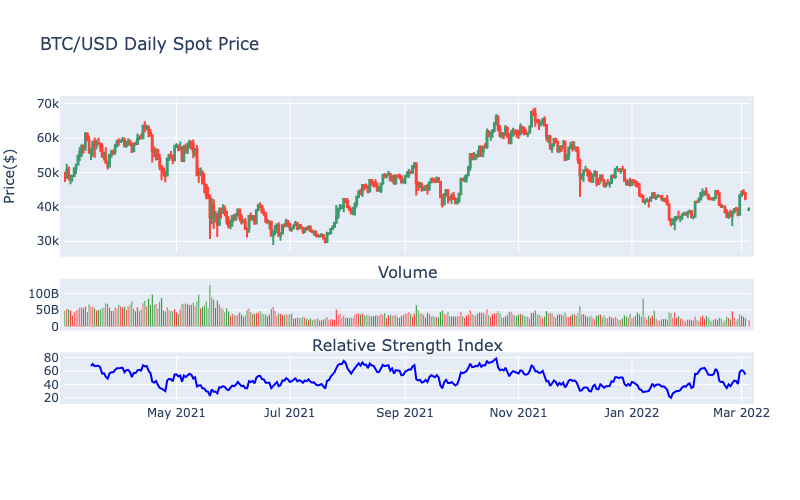
\includegraphics[width=0.9\textwidth]{RSI.png}
\end{center}

\caption{\textit{ Candlestick graph of daily spot price of BTC/USD from March 2021 to March 2022 with a subplot containing  RSI}}

\end{figure}

\section{Aroon Indicator}

Aroon indicator is used for trend reversal identification and a measure of its strength. Indicator is composed out of two lines aroon up and aroon down that measure the time between new highs or lows respectively. Alternatively, they measure the strength of a bullish or bearish trend. Obviously the main idea of the indicator is based upon the fact that bullish trends are naturely formed by subsequently creating new highs while bearish trends form new lows. Aroon Up and Aroon Down are computed as follows:

\begin{equation}
Aroon Up = \frac{25 - h}{25} * 100
\end{equation}
 
\begin{equation}
Aroon Down = \frac{25 - l}{25} * 100
\end{equation}

Where $h$ represents the number of periods from the last 25-period High and $l$ the number of periods from last 25-period Low. 

The interpretation of the indicator is very intuitive since the situation in which the Aroon Up line is above Aroon Down line signals bullish trend and when these two lines cross the signal of the trend reversal is generated. That also implies that for higher values of Aroon Up the bigger the strength and for lower values the uptrend is weaker and vice versa. In practice the crossover of these two lines is what generates the buy or sell signals, i.e. if Aroon Up crosses Aroon Down line from below a buy signal is generated and vice versa. 

Although, Figure 2.4 graphically illustrates the Aroon Up and Down lines well, it is simpler to transform these two lines into one oscillator that would produce buy or sell signal in the case of zero crossover from above and from below. That is achieved by subtracting Aroon Up and Aroon Down line creating Aroon Oscillator.


\begin{figure}[h]

\begin{center}
	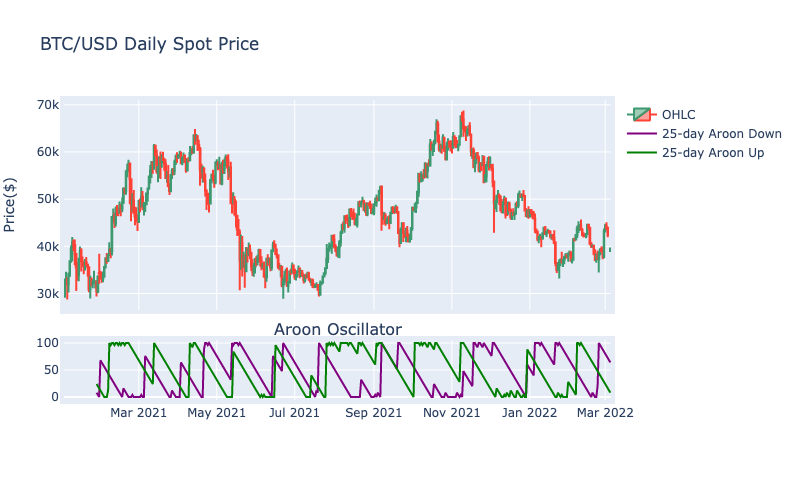
\includegraphics[width=0.9\textwidth]{Aroon.png}
\end{center}

\caption{\textit{ Candlestick graph of daily spot price of BTC/USD from March 2021 to March 2022 with subplots containing two lines for Aroon Up/Down Indicator and Aroon Oscillator}}

\end{figure}


\newpage


\section{Kalman Filters}


--




